\chapter{Appendix}

\section{Geometric Approach}

\todo[inline]{Explain why this idea is \enquote{dead}. Move to possible appendix because it is sill a nice connection between time series analysis and convex geometry?}

In this section, we study how the geometry of the point cloud $\mathcal{P}_k\subseteq\mathbb{R}^{k}$ changes with increasing embedding dimension $k$. For simple innovation distributions, like uniform or normal, the point cloud $\mathcal{P}_k$ is characterized by well known convex--geometric objects. The question becomes if we can apply some convex--geometric functional $f$ to these well known objects and detect a transition at $k=p+1$, where $p$ is the AR order of the embedded time series.

In order to be able to talk about the \enquote{geometry of a point cloud} in a rigorous way, we first need to introduce some concepts from probability theory. Let $Y$ be a $d$-dimensional random vector with density $f_Y$. The \textit{support} of $Y$ is given by
\begin{align*}
    \operatorname{supp}(Y)=\{x\in\mathbb{R}^k:\mathbb{P}(Y\in B_r(x))>0\text{ for all }r>0\}.
\end{align*}
In the case where $f_Y$ is continuous, it holds $\operatorname{supp}(Y)=\operatorname{cl}\{y\in\mathbb{R}^{k}:f_Y(y)>0\}$. The \textit{minimum volume set} (compare~\cite{JMLR:v7:scott06a}) is defined by
\begin{align*}
    E_{\alpha}\in\arg\min\{\lambda_d(A):\mathbb{P}(Y\in A)\ge\alpha,A\in\mathcal{B}(\mathbb{R}^d)\}.
\end{align*}
The \textit{highest density region} $C_{\alpha}$, $\alpha\in(0,1)$ (see~\cite{Hyndman01051996}) is defined by
\begin{align*}
    C_{\alpha}&=C_{h_{\alpha}}\\
    C_h&=\{x\in\mathbb{R}^{d}:f(x)\ge h\}\\
    h_{\alpha}&=\sup\{h\in\mathbb{R}:\mathbb{P}(Y\in C_h)\ge 1-\alpha\}
\end{align*}

\todo[inline]{connect these concepts with each other}

Let $X_t=\sum_{j=0}^{\infty}\psi_j Z_{t-j}$ be the MA($\infty$)-representation of an AR($p$) process, where $(Z_t)$ are the independent and identically distributed innovations with cumulative distribution function $F_0$ and where the sequence $(\psi_j)_{j\in\mathbb{N}_0}$ is defined recursively by $\psi_{-(p-1)}=\dots=\psi_{-1}=0$, $\psi_0=1$ and $\psi_j=\phi_1\psi_{j-1}+\dots+\phi_p\psi_{j-p}$ for all $j\ge 1$. Now each point $Y_t^{(k)}\in\mathcal{P}_k$ can be written as
\begin{align*}
    Y_{t}^{(k)}&=\begin{pmatrix}
        X_t\\
        X_{t-1}\\
        \vdots\\
        X_{t-k+1}
    \end{pmatrix}=\sum_{j=0}^{\infty}g_j^{(k)}Z_{t-j},
\end{align*}
where $g_j^{(k)}=(\psi_j,\psi_{j-1},\dots,\psi_{j-k+1})^{T}$. We have $\lim\limits_{j\to\infty}\psi_j=0$.

\todo[inline]{Explain/ Prove convergence of $(\psi_j)$ give convergence speed result. Connect to stationarity/ causality, obtain some kind of upper bound for $|\psi_j|$}

Consider the case $k\ge 
p+1$. The AR relation allows us to write
\begin{align}\label{eq:ar_relations}
    X_{t-j}-\phi_1X_{t-j-1}-\dots-\phi_pX_{t-j-p}=Z_{t-j}, && j=0,1,\dots,k-p-1
\end{align}

Since innovations $(Z_t)$ are centered, the points $Y_t^{(k)}$ lie around the hyperplane $\{x_0-\phi_1x_{1}-\dots-\phi_px_p=0:(x_0,\dots,x_p)\in\mathbb{R}^{p+1}\}$. Note that the intersection of the $k-p$ central hyperplanes can be written as
\begin{align*}
    L_k&:=\bigcap_{j=0}^{k-p-1}\left\{(x_0,\dots,x_{k-1})\in\mathbb{R}^k:x_j-\phi_1x_{j+1}-\dots-\phi_px_{j+p}=0\right\}\\&
    =\operatorname{Im}(A)
\end{align*}
where the $k\times p$-matrix $A$ has rank $p$.

\subsection{Uniformly distributed innovations}

\begin{Def}[Minkowski sum]
    Let $A$ and $B$ be two subsets of a vector space $V$. Their Minkowski sum is given by the set $A+B=\{a+b:a\in A,b\in B\}$.
\end{Def}

\begin{Def}[Hausdorff distance]
    Let $(M,d)$ be a metric space and $X,Y$ two nonempty subsets of $M$. The Hausdorff distance $d_H$ between $X$ and $Y$ is defined by
    \begin{align*}
        d_H(X,Y)=\sup_{w\in M}|d(w,X)-d(w,Y)|,
    \end{align*}
    where $d(w,X)=\inf\{d(w,x):x\in X\}$.
\end{Def}

\begin{Def}[Zonotope]
    A zonotope is the Minkowski sum of finitely many line segments. It is said to be generated by $w_1,\dots,w_n\in\mathbb{R}^d$ if it has the form
    \begin{align*}
        \left\{a_1w_1+\dots+a_nw_n:0\le a_j\le 1\text{ for all }j\right\}
    \end{align*}
\end{Def}

\begin{Def}[Zonoid]\label{def:zonoid}
    Let $w=(w_n)_{n\in\mathbb{N}_0}$ be a sequence of vectors in $\mathbb{R}^d$. A set $\mathcal{Z}$ is called a zonoid generated by $w$ if $d_H(\mathcal{Z},\mathcal{Z}_n)\to0$ for $n\to\infty$, where $\mathcal{Z}_n$ is a zonotope generated by $w_0,w_1,\dots,w_n$.
\end{Def}

Let $(Z_t)\sim\mathcal{U}[-1,1]$. Then the support of $Y_t^{(k)}$ is given by a zonoid $\mathcal{Z}^{(k)}$ generated by $(g_j^{(k)})_{j\in\mathbb{N}_0}$. By Definition~\ref{def:zonoid} $\mathcal{Z}^{(k)}$ can be approximated arbitrarily closely by the zonotope $Z_n^{(k)}$ generated by $g_0^{(k)},\dots,g_n^{(k)}$. This object has (at most) $2^{n+1}$ corner points. For visualization, see Figure~\ref{fig:zonotopes}.

\begin{figure}[ht]
  \centering

  \begin{minipage}[b]{0.32\textwidth}
    \centering
    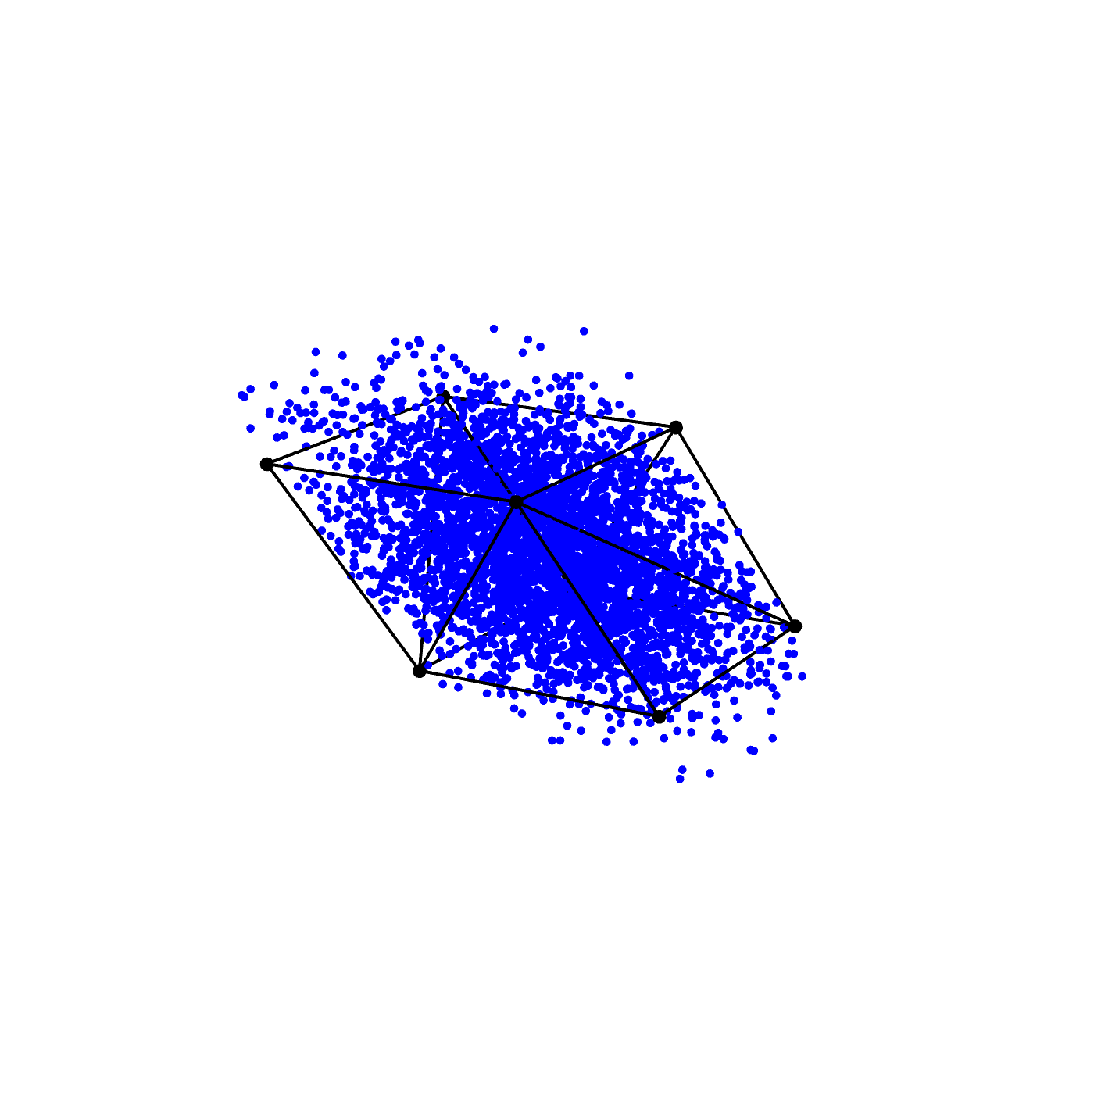
\includegraphics[width=\textwidth]{Abschlussarbeit_2021/LaTeX/images/zonotope_approximation_n3.pdf}
  \end{minipage}\hfill
  \begin{minipage}[b]{0.32\textwidth}
    \centering
    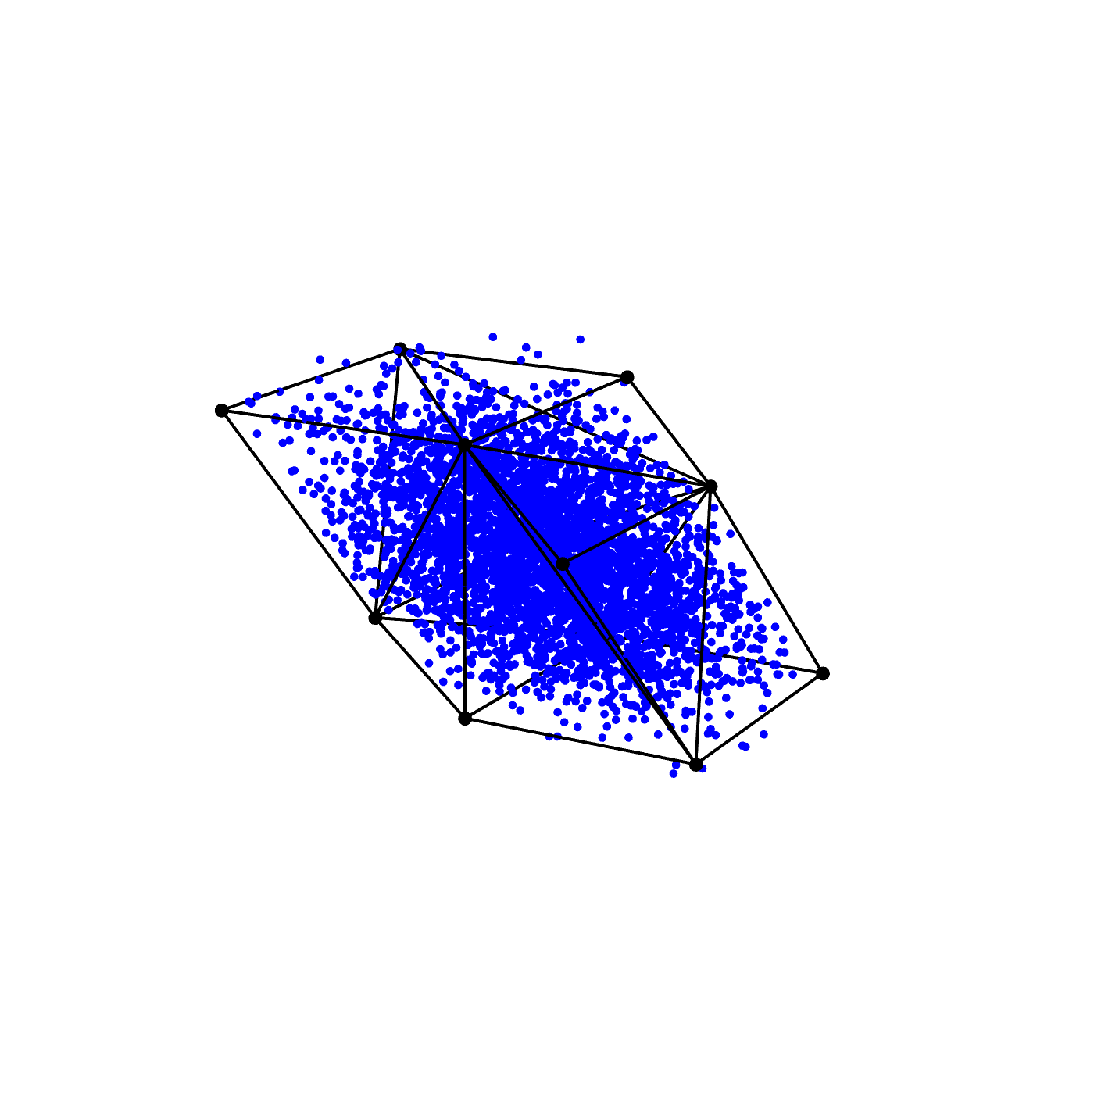
\includegraphics[width=\textwidth]{Abschlussarbeit_2021/LaTeX/images/zonotope_approximation_n4.pdf}
  \end{minipage}\hfill
  \begin{minipage}[b]{0.32\textwidth}
    \centering
    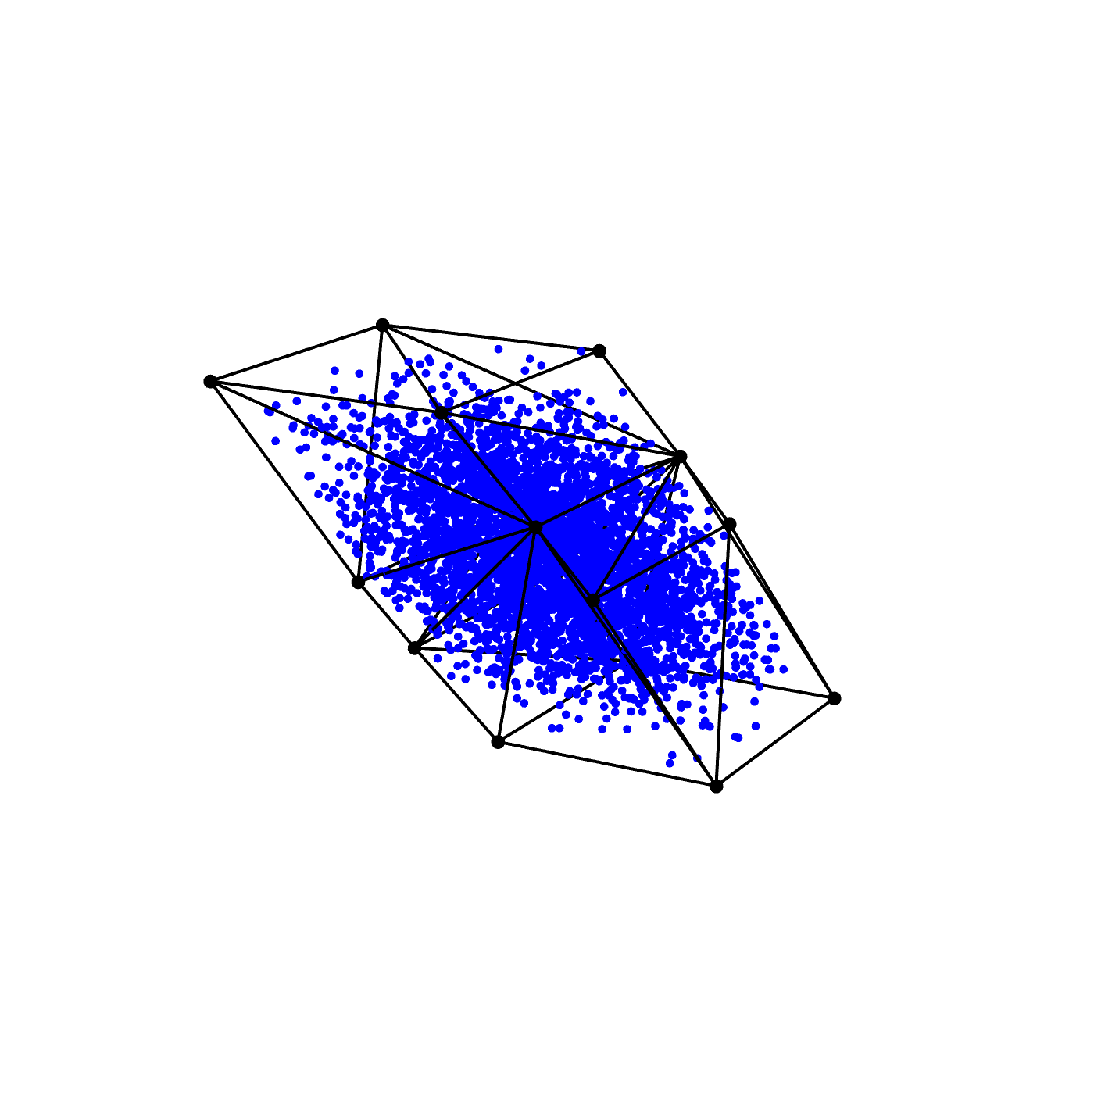
\includegraphics[width=\textwidth]{Abschlussarbeit_2021/LaTeX/images/zonotope_approximation_n5.pdf}
  \end{minipage}

  \caption{Zonotopes approximating the zonoid $\mathcal{Z}$, where $n=3$ (left), $n=4$ (center) and $n=5$ (right)}
  \label{fig:zonotopes}
\end{figure}

\todo[inline]{give approximation quality statement which should connect to the sequence $\psi_j$}

\todo[inline]{Formula for corner points?}

In the case of uniform innovations $Z_t\sim\mathcal{U}[-1,1]$ the points also lie between the hyperplanes with the same form as the central hyperplane, but with affine parts $-1$ and $1$. See Figure~\ref{fig:3d_emb_ar2}.

\begin{figure}[ht]
    \centering
    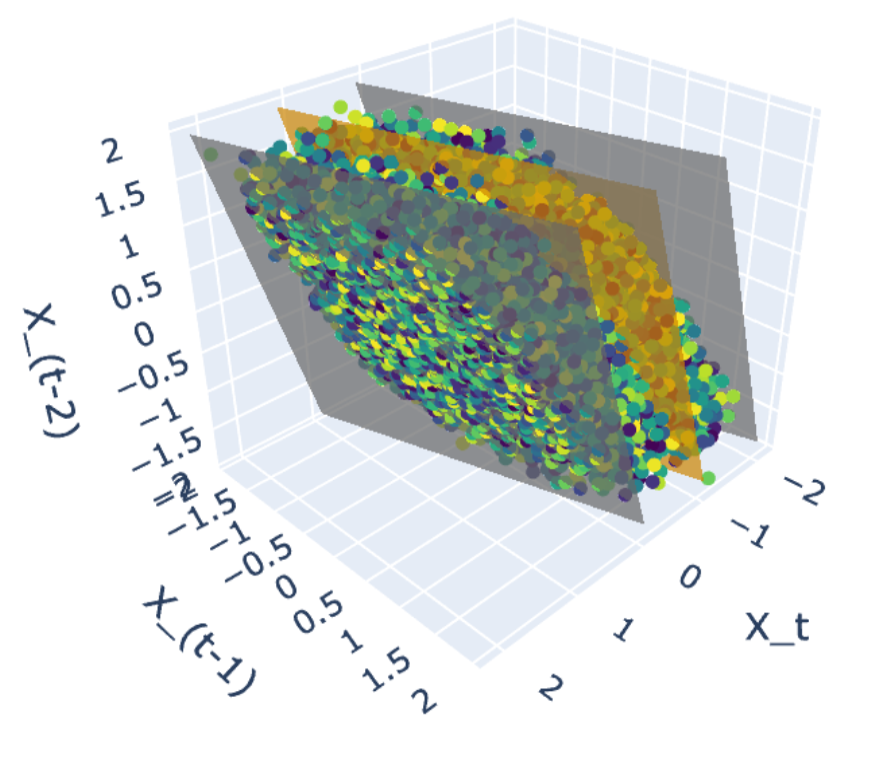
\includegraphics[width=0.5\linewidth]{Abschlussarbeit_2021/LaTeX/images/3d_emb_ar2_cropped.png}
    \caption{Sliding-window embedding ($k=3$) of an AR(2) process. The orange plane is the central plane (right side = 0), the two gray planes are the planes with affine parts -1 and 1 (due to the innovations being $\mathcal{U}[-1,1]$ distributed)}
    \label{fig:3d_emb_ar2}
\end{figure}

If $k>p+1$, the point $Y_t^{(k)}$ lies inside the intersection of multiple slabs:
\begin{align*}
    &\left\{(x_0,\dots,x_{k-1})\in\mathbb{R}^{k}:\begin{array}{l}
    -1\le x_j-\phi_1x_{j+1}-\dots-\phi_px_{j+p}\le 1,\\
    j=0,\dots,k-p-1 
    \end{array}\right\}\\&
    \bigcap_{j=0}^{k-p-1}\left\{(x_0,\dots,x_{k-1})\in\mathbb{R}^{k}:-1\le x_j-\phi_1x_{j+1}-\dots-\phi_px_{j+p}\le 1\right\}
\end{align*}

\todo[inline]{Set $p=1$ and $k=3$, visualize the intersection of slabs}

The distance between the two restricting hyperplanes is given by the formula
\begin{align*}
    d=\frac{2}{\sqrt{1+\phi_1^2+\dots+\phi_p^2}}
\end{align*}

\begin{Def}[Support function]
    Let $K\subseteq\mathbb{R}^{d}$ be a convex nonempty set. The support function of $K$ is $h_K:\mathbb{R}^d\to\mathbb{R}$, $h_K(u)=\sup\{\langle x,u\rangle:x\in K\}$.
\end{Def}

A convex body is a compact nonempty convex set. 

\begin{Lem}
    Let $K,L\subseteq\mathbb{R}^d$ be two convex bodies. Then
    \begin{align*}
        d_H(K,L)=\sup_{u\in S^{d-1}}|h_{K}(u)-h_{L}(u)|.
    \end{align*}
\end{Lem}

The support function of a zonotope is particularly easy: $h_{\mathcal{Z}_n^{(k)}}(u)=\sum_{j=0}^{n}|\langle g_j^{(k)},u\rangle|$. The width in direction $u$ is given by
\begin{align*}
    w_k(u)=h_{\mathcal{Z}_n^{(k)}}(u)+h_{\mathcal{Z}_n^{(k)}}(-u)=2h_{\mathcal{Z}_n^{(k)}}(u)
\end{align*}
Consider the case $k\ge p+1$. We have
\begin{align*}
    m_k=\min_{u\in S^{k-1}}w_k(u)=\frac{2}{\sqrt{1+\phi_1^2+\dots+\phi_p^2}}
\end{align*}
This minimum is attained at the finite set of points
\begin{align*}
    \left\{\pm\frac{q_r^{(k)}}{\|q_{\phi}\|_2}:r=0,\dots,k-(p+1)\right\}
\end{align*}
where $q_{\phi}=(1,-\phi_1,\dots,-\phi_p)$ and
\begin{align*}
    q_r^{(k)}=(\underbrace{0,\dots,0}_{r},1,-\phi_1,\dots,-\phi_p,0,\dots,0)\in\mathbb{R}^{k}
\end{align*}

\todo[inline]{What about $k<p+1$? Is $\min w_k(u)>2^{-1}\sqrt{1+\phi_1^2+\dots+\phi_p^2}$}

The relation $k\mapsto\min w_k(u)$ has a kink at $k=p+1$. The downside is that one needs to estimate the coefficients $\phi_1,\dots,\phi_r$ for different candidate orders $r$.

An empirical version is given by
\begin{align*}
    w_k(u)&=\sup\{\langle x,u\rangle: x\in \mathcal{Z}_n^{(k)}\}-\inf\{\langle x,u\rangle:x\in\mathcal{Z}_n^{(k)}\}\\
    \hat{w}_k(u)&=\max_{t}\langle u,Y_t^{(k)}\rangle-\min_{t}\langle u,Y_t^{(k)} \rangle=\max_{x\in\mathcal{P}_k}\langle u, x\rangle-\min_{x\in\mathcal{P}_k}\langle u,x\rangle\\
    \hat{m}_k&=\min_{u\in S^{k-1}}\hat{w}_k(u)
\end{align*}

\todo[inline]{Give some convergence result $\hat{w}_k(u)\to w_k(u)$ or $m_k\to\hat{m}_k$}

The idea is to minimize $\hat{w}_k(u)$ over all $u\in S^{k-1}$ and examine the relation $k\mapsto \hat{m}_k$.

How is $\hat{w}_k(u)$ minimized? The naive idea is the following: sample many directions $u_1,\dots,u_M$ and set $\min\limits_{j=1,\dots,M}\hat{w}_k(u_j)\approx\hat{m}_k$.

\cite{10.1145/1008731.1008736} give a method to construct a smaller subset $\mathcal{Q}_k\subseteq\mathcal{P}_k$ such that
\begin{align*}
    (1-\epsilon)\hat{w}_k(u)\le\max_{x\in\mathcal{Q}_k}\langle u, x\rangle-\min_{x\in\mathcal{Q}_k}\langle u,x\rangle \le\hat{w}_k(u)
\end{align*}
This gives a computational advantage, as we do not have to compute $\langle u,x\rangle$ for all $x\in\mathcal{P}_k$ but only for all $x\in\mathcal{Q}_k$.

\begin{figure}[ht]
    \centering
    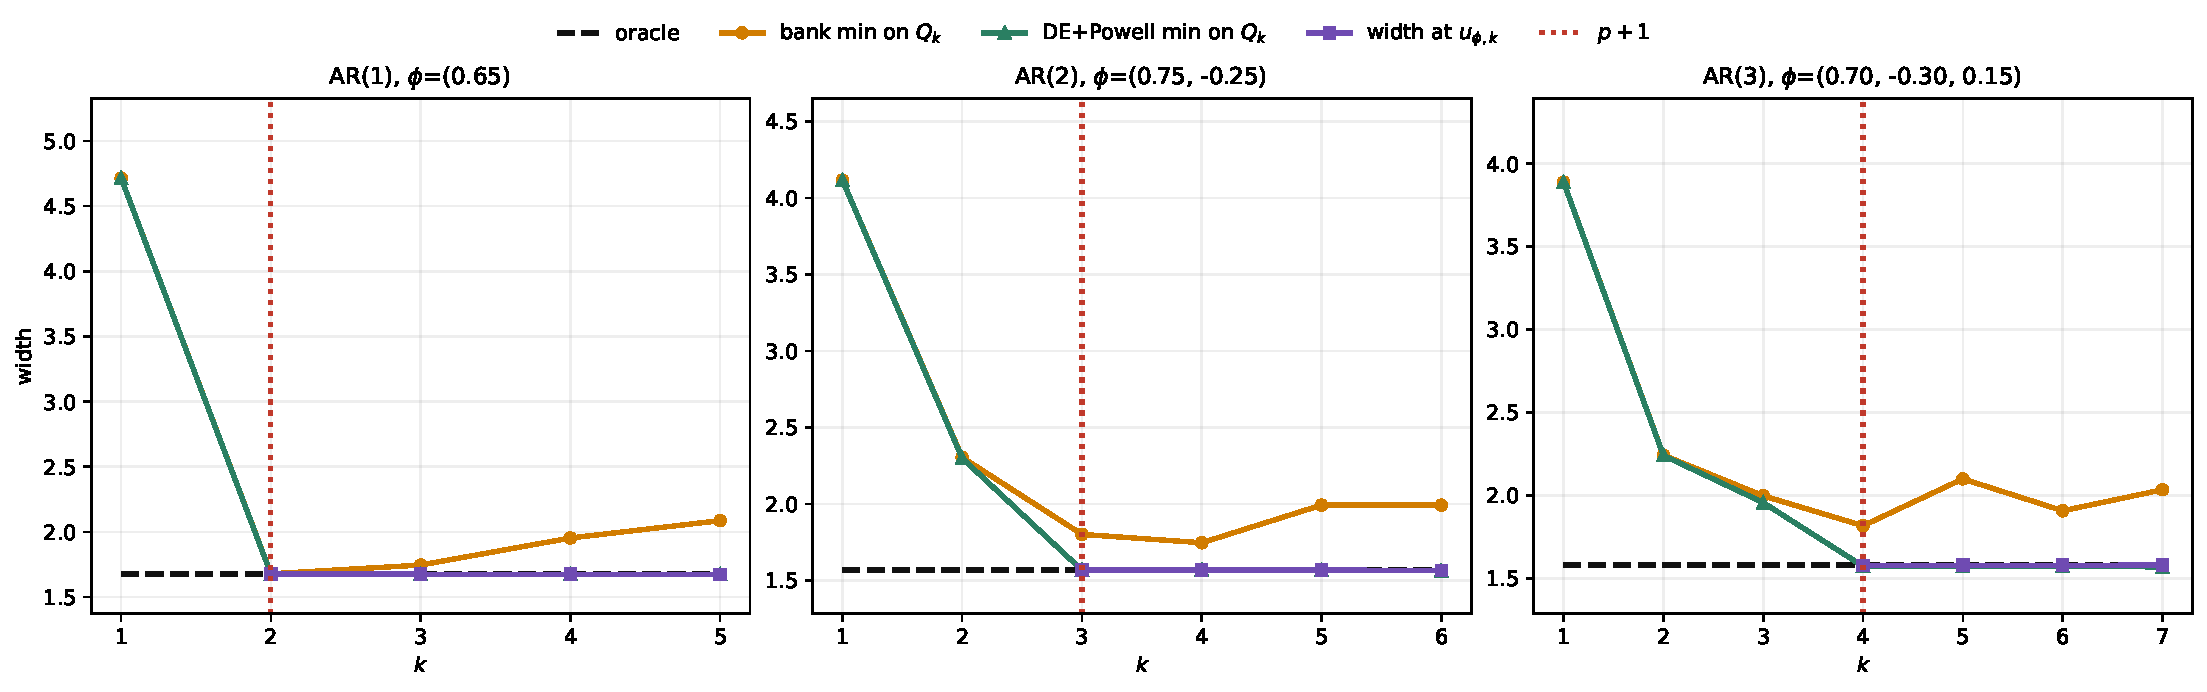
\includegraphics[width=\linewidth]{Abschlussarbeit_2021/LaTeX/images/ar_min_width_four_curve_direction_bank_diagnostic_p123.pdf}
    \caption{Caption}
    \label{fig:placeholder}
\end{figure}

\todo[inline]{show numerical results for $p=1,2,3,\dots$}
\todo[inline]{compare $k\mapsto\min w_k(u)$ and $k\mapsto\min\hat{w}_k(u)$}

\subsection{Normally distributed innovations}

Next, we turn our attention to Gaussian innovations, which is often seen as the default case, that is, $Z_t\sim N(0,\sigma^2)$ for some $\sigma>0$. Using the MA($\infty$) representation, we see that $Y_t^{(k)}\sim\mathcal{N}(0,\Gamma_k)$ with covariance matrix
\begin{align*}
    \Gamma_k=\sigma^2\sum_{j=0}^{\infty}g_j^{(k)}(g_j^{(k)})^{T}
\end{align*}
The covariance matrix plays an important role in describing the geometry of the point cloud $\mathcal{P}_k$. Let $E_c=\{y\in\mathbb{R}^k:y^{T}\Gamma_k^{-1}y\le c\}$ be the ellipsoid of size $c>0$. Then for all $\alpha\in(0,1)$ we have
\begin{align*}
    E_{c_{\alpha}}\in\arg\min\left\{\operatorname{Vol}(A):\mathbb{P}(Y\in A)\ge\alpha:A\subseteq\mathbb{R}^{k}\right\}
\end{align*}
That is, the ellipsoid with size $c_{\alpha}$ is the set with minimum volume, such that the probability that $Y$ is inside $E_{c_{\alpha}}$ is at least $\alpha$.

\todo[inline]{find reference or prove}

\subsection{Intrinsic Volumes}

\todo[inline]{Handbook of Convex Geometry}

We have a zonotope $Z^{(n)}_k=\sum_{j=0}^{n}g_j[-1,1]$ with \textcolor{red}{unknown} vectors $g_j\in\mathbb{R}^k$. Here, $k$ is the embedding dimension. The $j$-th quermassintegral of $Z^{(n)}_k$, denoted by $W_j(Z^{(n)})$ are defined as coefficients that fulfill
\begin{align*}
    \operatorname{Vol}(Z^{(n)}_k+tB)=\sum_{j=0}^{k}\binom{k}{j}W_j(Z^{(n)}_k)t^{j}
\end{align*}
where $B=B(0,1)=\{x\in\mathbb{R}^k:\|x\|\le1\}$. The $j$-th intrinsic volume is defined by
\begin{align*}
    V_j(Z^{(n)}_k)=\binom{k}{j}\frac{W_{k-j}(Z^{(n)}_k)}{\kappa_{k-j}}, && j=1,\dots,k
\end{align*}
It can be shown that the $j$-th intrinsic volume can by computed by the formula
\begin{align*}
    V_j(Z^{(n)}_k)=2^{j}\sum\limits_{I\subseteq\{0,\dots,n\},|I|=j}\sqrt{\det{(G_I^TG_I)}}
\end{align*}

\todo[inline]{Big Question: How to generalize this approach for a wide class of innovation distributions? We only get the nice zonotope formulas because of uniform innovations}

\todo[inline]{Maybe find a class of distributions where the highest density region (or minimum volume set) has a nice geometric shape and compute the intrinsic volumes of that shape}





\subsection{Numerical Results}

\begin{itemize}
    \item AR($p$) for $p=1,2,3$
    \item different innovations
    \item compare with classical order selection
    \item finite sample stability $(X_1,\dots,X_T)$, $T=200,500,1000$
\end{itemize}